

\newpage
\subsection{Die Dipol Antenne}\label{sec:DipolAntenne}
Der zentral gespeiste Dipol besteht meistens aus zwei runden Leiterstäben mit dem Durchmesser $d$ und der Länge $l$. Die beiden Stäbe haben eine gesamte Länge von $2l$. Die  Stäbe liegen so aneinander, dass in der Mitte der beiden Stäbe eine kleine Lücke entsteht. Die gesamte Länge der beiden Stäbe ist viel grösser als  der Durchmesser $d$. Wird eine Spannung  in der Lücke zwischen den beiden Stäben angelegt, kommt es zu einer Stromverteilung über die gesamte Länge der  Stäbe. Oft wird die Spannung mit einer Zweidrahtleitung,  diese wird englisch \textit{Transmission Line} genannt, zwischen den Leiterstäben angebracht. Die anschliessende Stromverteilung der beiden runden Leiterstäbe liefert den Ursprung der Wellenausbreitung. In erster Näherung kann die sich von der Speisestelle ausbreitende Welle als richtungsunabhängige Kugelwelle betrachtet werden \cite{elliott1981antenna}.
%E^j(wt-kr)/4pimu^-1 r
%Elliot Seite 29 Nr1.93

\begin{equation}\label{term:Kugelwelle}
\frac{e^{j(\omega t-kr)}}{4\pi \mu_{0}^{-1}r}
\end{equation}
\todo{Nr1.93 Elliott Formel}

%%%%%%%%%%%%%%%%%%%%%%%%%%%%%%%%%%%%%%%%%%%%%%%%%%%%%%%%%%%%%%%%%%%
\begin{figure}[!h]
	\centering
	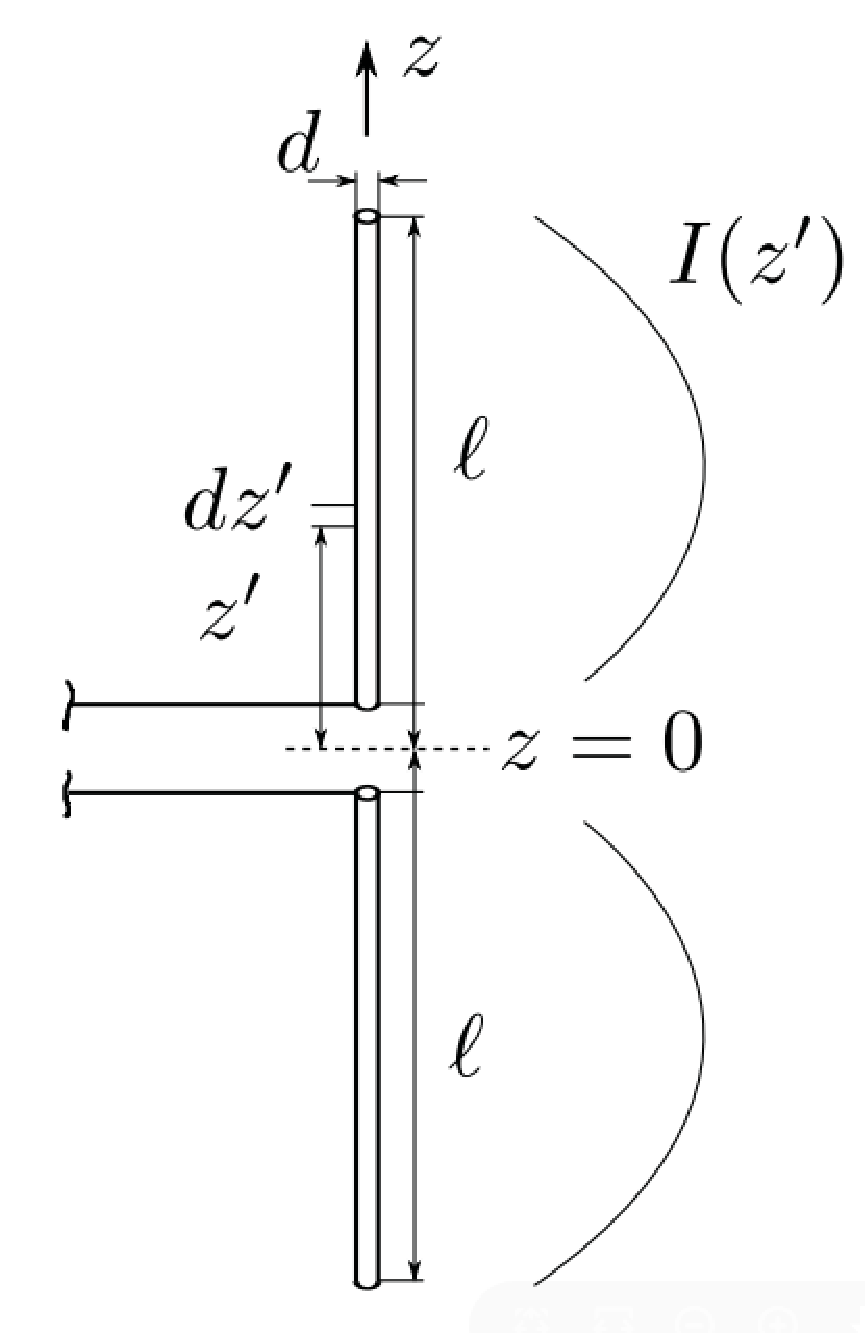
\includegraphics[width=4cm]{content/bilder/Dipol_EMANT_S42.pdf}%
	\caption{Dipol Antenne mit Stromverteilung \cite{Tekom}}
	\label{FitzDipol}
\end{figure}
%%%%%%%%%%%%%%%%%%%%%%%%%%%%%%%%%%%%%%%%%%%%%%%%%%%%%%%%%%%%%%%%%%%

Die Stromausbreitung in der Dipol Stabantenne entspricht der Stromverteilung einer am Ende offenen Zweidrahtleitung. Deren Enden im $90^\circ$ abgewinkelt werden. Das offene Ende der Leitung führt zu einer Reflexion der zuführenden Welle in die umgekehrte Richtung und somit zu einer stehenden Welle in der Leitung. Stromführende Elemente, die nahe beieinander liegen, deren Amplituden gleich aber gegenläufig sind, strahlen nur gering. Dies sind Eigenschaften einer guten Zweidrahtleitung. Aber die voneinander abgewinkelten Leitungsenden strahlen stark.
Als Näherung für die Stromverteilung soll folgendes gelten \cite{elliott1981antenna}:
\begin{equation}\label{I_xt_Dipol} 
I(x,t) =I_{m}sin([k(l-x)])e^{j\omega t}
\end{equation}
%Elliot Seite 59 Formel 2.1
\todo{S59 Formel 2.1}
Aus Formel \ref{I_xt_Dipol} kann entnommen werden, dass sich der Strom entlang der Dipolarme ändert. Die Stromverteilung ist somit vom Betrachtungsort $x$ und Zeitpunkt $t$ abhängig.


Bei einem Dipol mit dem Durchmesser $d<<\lambda$ wird dieser zu einem dünnen Stromfaden. Die Stromdichte im Leiter kann \textbf{J}\textit{d}\textbf{\textbf{V}} mit \textbf{I}\textit{d}\textbf{\textbf{l}} als Stromelement ersetzt werden. Die Summe der Elementardipole mit konstantem Strom können als Quelle betrachtet werden \cite{elliott1981antenna}.\\

\begin{equation}
I_{m}sin(k(l-dz))
\end{equation}
%Elliot Seite 61 Formel 2.2
Die hier beschriebe Antenne hat einen so kleinen Durchmesser verglichen mit ihrer Länge L, dass der Stromfaden nur eine Ausdehnung entlang der z Achse aufweist. Die Gewichtungsfunktion dieser Summe von Elementardipolen die alle in der z Achse liegen ist:\\
$a(\varphi)= 0$
jedoch die Gewichtungsfunktion in $\theta$ Richtung beträgt nach R. Elliott \cite{elliott1981antenna}:
\begin{equation}\label{eq:Gewichtungsfunktion}
a_{\theta}(\theta)=- \frac{2I_{m}}{k sin(\theta)} \lbrack cos(kl cos(\theta)) - cos(kl) \rbrack
\end{equation}
%Elliot Formel 2.6 oder Joss EMANT 122.

Es sollen zwei Fälle genauer betrachtet werden.
\begin{itemize}
\item der Halbwellendipol mit 2l= $\lambda/2$
\item der kurze Dipol mit 2l$<<\lambda$
\end{itemize}
\subsubsection{Der Halbwellendipol}
Der $\lambda/2$ Dipol ist eine der wichtigsten Antennen. Über die Gewichtungsfunktion in Formel \ref{eq:Gewichtungsfunktion} und dem Term der sich ausbreitenden Kugellwelle \ref{term:Kugelwelle} lässt sich auf das Fernfeldverhalten schliessen \cite{elliott1981antenna}.
\begin{equation}
E_{\theta}=j60I_{m} \frac{e^{j(\omega t - kr)}}{r} \lbrack \frac{cos\lbrack  (\pi/2) cos(\theta)\rbrack}{sin(\theta)} \rbrack
\end{equation}
\begin{equation}
H_{\phi}=j \frac{I_{m}}{2\pi} \frac{e^{j(\omega t - kr)}}{r} \lbrack \frac{cos\lbrack  (\pi/2) cos(\theta)\rbrack}{sin(\theta)} \rbrack
\end{equation}
%E(theta)= Ellito 2.8
%E(phi) = Ellito 2.9

Die Feldverteilung kann in der  Zweidimensionalen Polar Form oder in einer Dreidimensionalen Feldverteilung dargestellt werden.
Die nachfolgende Grafik zeigt eine E Feldverteilung als Schnitt durch die xz Ebene.\\
%!!!!Wichtig!!!!!Bild aus Matlab importieren\\
\todo{Matlab Bild der Feldausbreitung}

%%%%%%%%%%%%%%%%%%%%%%%%%%%%%%%%%%%%%%%%%%%%%%%%%%%%%%%%%%%%%%%%%%%
\begin{figure}[h]
\begin{center}
\begin{tikzpicture}
	\draw (0,3) node at (0.5,0.5) {xz Ebene} -- (10,3);%Fadenkreuz horizontal
	\draw (5,0) -- (5,6);%Fadenkreuz vertikal
	\draw [line width=1mm] (5,3.2) -- (5,4.5);%upper arm
	\draw [line width=1mm] (5,1.5) -- (5,2.8);%lower arm
	\draw (3,3) circle (2cm);%linker Kreis
	\draw (7,3) circle (2cm);%rechter Kreis

	\node[draw] at (5,6.5) {$\theta=0$};
	\node[draw] at (8,5.5) {$E(\theta)$};

\end{tikzpicture}
\end{center}
	\caption{Das E Feld einer Dipolantenne in der xz Ebene}
	\label{fig:DipolEFerd}
\end{figure}

%%%%%%%%%%%%%%%%%%%%%%%%%%%%%%%%%%%%%%%%%%%%%%%%%%%%%%%%%%%%%%%%%%%


Dargestellt ist ein $\lambda/2$ Dipol der in z Richtung aufgerichtet ist. Es ist zu erkennen, dass bei $\theta = 0 ^\circ $  und $\theta = 180 ^\circ $ kein elektrisches Feld abgestrahlt wird. Stellt man sich die Grafik als um eine um $\varphi$ von 0 Grad bis 360 Grad rotierende Scheibe vor, so kommt die bekannte Doughnut Form zum Vorschein.

Die von $\vartheta$ und $\varphi$ abhängige Leistung ist gegeben durch \cite{elliott1981antenna}:
%P(theta,phi)= elliot2.10
\begin{equation}
P(\theta,\phi)=\frac{2\eta I_{m}^{2}}{(4\pi r)^{2}}\lbrack \frac{cos^{2}\lbrack (\pi/2) cos(\theta)\rbrack}{sin^{2}(\theta)}\rbrack
\end{equation}

%Durch Lösung des Doppelintegrals 
%Elliot Seite 63
Durch das Auflösen der Doppelintegrale über $\varphi$ von 0 bis $\pi$  und $\theta$ von 0 bis $\pi$ erhält man eine nummerische Lösung der Integrale über die gesamte Kugeloberfläche \cite{elliott1981antenna}:
\begin{equation}
P_{rad}=0.609 \frac{\eta I_{m}^{2}}{2\pi}
\end{equation}
%elliot 63 Forlmel 2.11

Wie die  Grafik \ref{fig:DipolEFerd} zeigt, ist die maximale Feldausbreitung auf der Höhe der Einspeisestelle bei $\theta = 90 ^\circ $ maximal,  denn der  $sin(90 ^\circ ) $ entspricht 1.
Der maximale Richtwert oder Richtfaktor,  aus dem englischen als \textit{directivity} bekannt, erhält man indem die Abgestrahlte Leistung mit einem isotropen Kugelstrahler verglichen wird\cite{elliott1981antenna}.
\begin{equation}
D(peak)=\frac{P(\theta,\varphi)(\pi/2)}{P_{rad}/ 4 \pi r^{2}} =1.64
\label{eq:Directivity}
\end{equation}
%Dmax=1.64 nach Ellito 2.12
Das besagt, dass die Abstrahlung in den Raum nicht homogen ist. Das Resultat des Richtfaktors für eine $\lambda /2$ Dipolantenne aus Gleichung \ref{eq:Directivity} ist ein Verhältnisfaktor. Dieser ist bezogen auf einen gleichmässig in den Raum strahlenden Kugelstrahler. Die Hauptkeule, ist die Richtung der grössten Abstrahlung ist also um den Faktor 1.64 grösser als bei einem Normstrahler. Der Richtfaktor wird oft in dB abgegeben. Da man sich auf den isotropen Strahler bezieht, ist die Angabe dBi und entspricht in dem gezeigten Beispiel $10\log{1.64}=2.15dBi$.\\

Bei einem Halbwellendipol der Länge 2l mit $l=\lambda/4 $ ist der Scheitelwert des Antennenstromes $I_{m}$ beim Einspeisepunkt, dem Zentrum des Dipol bei z= 0. Somit kann gesagt werden, dass die Zuleitung  die folgende Leistung  liefert:
%Elliot 2.14
\begin{equation}
P=\frac{1}{2} I_{m}^{2}R_{rad}=(0.609)\frac{\eta I_{m}^{2}}{2\pi}
\end{equation}

Der Strahlungswiderstand oder auch $R_{rad}$ genannt kann im Fall des $\lambda /2$ Dipol nummerisch als 73 Ohm bestimmt werden.
\begin{equation}\label{RradDipol}
R_{rad}=\frac{0.609 \eta}{\pi}= 73 Ohm
\end{equation}
